\chapter{Dirac Delta Function}
In mathematical models of physical systems we often come across functions that have finite or infinite discontinuities (Potential barriers, Impulse functions). Even though they dont belongs to the generalm definition of functions we can represent them as generalised function or distributions. The most common among them are the step function and the dirac delta function.
\section{The Step Function}
Let's start with the definition of the unit step function, $\theta(x)$ :
$$
\theta(x)=\left\{\begin{array}{ll}
0 & \text { for } x<0 \\
1 & \text { for } x>0
\end{array}\right.
$$
We do not define $\theta(x)$ at $x=0$. Rather, at $x=0$ we think of it as in transition between 0 and 1 .The function is called the unit step function because it takes a unit step at $x=0$. It is sometimes called the \textbf{Heaviside function}. The graph of $\theta(x)$ is simple.
It is obvious that $\theta(x)$ has a finite jump at $x=0$. It is sometimes convenient to define $\theta(0)$ to be the average value $\frac{1}{2}$, but this is not always necessary.
\begin{align*}
\text{The sum } \ \theta(x)+\theta(-x)&=1\\
\text{The difference}\ \theta(x)-\theta(-x)&=\varepsilon(x)
\end{align*}
Where, $\varepsilon(x)$ is the signum function.
\begin{equation}
\varepsilon(x)=\left\{\begin{array}{rr}
+1 & \text { for } x>0 \\
-1 & \text { for } x<0 \\
0 & \text { for } x=0
\end{array}\right.
\end{equation} The function $\varepsilon(x)$ looks like the limit of a tanh (or hyperbolic tangent) function as the 'kink' in the function becomes more and more steep, i.e., as the slope at the origin tends to infinity, as shown in Figure.\ref{Dirac delta} In fact, we could define $\varepsilon(x)$ as the limit of a continous sequence of functions $\tanh(\frac{x}{\varepsilon(x)})$.
\begin{figure}[H]
	\centering
	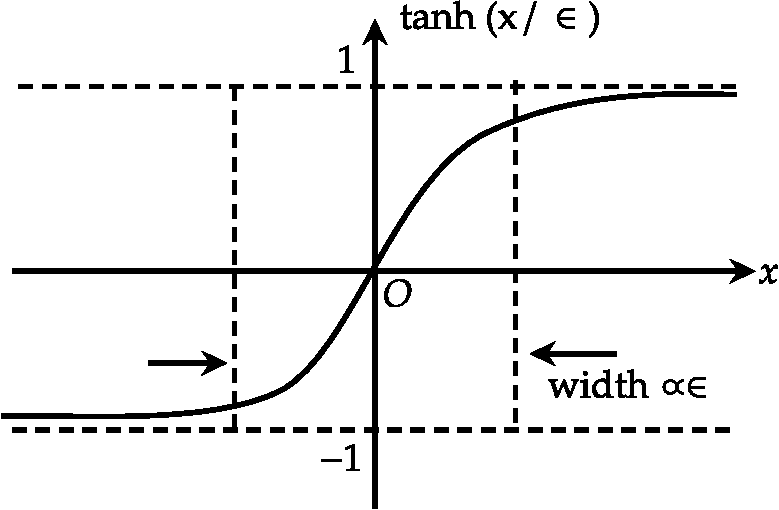
\includegraphics[height=4cm,width=5cm]{unit step function}
	\caption{The function of $ \tanh{(x/\epsilon)} $}
	\label{Dirac delta}
\end{figure}
\section{Dirac Delta Function}
\subsection{Kronecker delta $\delta$}
let us consider a sequence $\left(a_{1}, a_{2}, \ldots\right)=\left\{a_{j} \mid j=1,2, \ldots\right\} .$ How do we select a particular member $a_{i}$ from the sequence? We do so by summing over all members of the sequence with a selector called the \textbf{Kronecker delta}, denoted by $\delta_{i j}$ and defined as
$\delta_{i j} \stackrel{\text { def. }}{=}\left\{\begin{array}{ll}1 & \text { if } i=j \\ 0 & \text { if } i \neq j\end{array}\right.$
It follows immediately that
\begin{align*}
\sum_{j} \delta_{i j} a_{j}&=a_{i}\\
\sum_{j} \delta_{i j}&=a_{i}\qquad \text{For each value of } \ i\\
\delta_{i j}&=\delta_{j i} \qquad \text{Symmetry property. }
\end{align*}
Now if  we have a continuos function, we must replace the summation over  $j$ by an integration over $x$. The role of the specified index $i$ is played by the specified point $a$. The analog of the Kronecker delta is written like a function, retaining the same symbol $\delta$ for it. So we seek a `function' $\delta\left(x-a\right)$ such that
\begin{equation}
\int_{-\infty}^{\infty}  \delta\left(x-a\right) f(x) d x=f\left(a\right)
\end{equation}
Exactly as in the discrete case of the Kronecker delta, we impose the normalization and symmetry properties,
\begin{equation}
\int_{-\infty}^{\infty} \delta\left(x-a\right) d x=1 \quad \text { and } \quad \delta\left(x-a\right)=\delta\left(a-x\right)
\end{equation}
 $\delta\left(x-a\right)$ is more like the kernel of an integral
 \begin{equation}
 \int_{-\infty}^{\infty} \delta\left(x-a\right) d x=0 \quad \text { if } \quad x \neq a \quad \text{Or the limit of integration excludes the point `$a$'} 
 \end{equation}
 \section{Various representations of Delta function}
 Let us consider a rectangular fuunction defined as,
 \begin{equation}
R_{\varepsilon} =\left\{\begin{array}{ll} \frac{1}{2\varepsilon} & x-\varepsilon < x< x+2\varepsilon \\ 0 & \text{Otherwise }\end{array}\right. 
 \end{equation} 
 We can consider  this as a rectangular window of width $2\varepsilon$ and height $\frac{1}{2\varepsilon}$

